\section{Training Setup}
\label{app:training_setup}

% Appendix snippet. Expected packages in the main paper:
% \usepackage{booktabs}
% \usepackage{array}
% \usepackage{amsmath,amssymb}

\subsection{Tasks and Algorithm Grid}

Paper experiments use five seeds $\{7,8,9,10,11\}$.
Experiment grid contains three simulation backends and seven algorithms.

\begin{table}[h]
\centering
\small
\setlength{\tabcolsep}{5pt}
\caption{Paper-core benchmark grid.}
\label{tab:appendix-paper-core-grid}
\begin{tabular}{p{0.18\linewidth}p{0.64\linewidth}c}
\toprule
Backend & Tasks & Count \\
\midrule
Air Hockey & puck-goal position, $r=0.06$, observation mode=velocity / real-transfer-history & 2 \\
Box2D & center, goal, hard, hard-velocity, maze & 5 \\
MetaWorld & push, pick-place, peg-insert-side, sweep-into & 4 \\
\midrule
Algorithms & PPO, SAC, SAC+HER, SAC+HINT, CRL, CRTR, IWR & 7 \\
\bottomrule
\end{tabular}
\end{table}

% \begin{table}[h]
% \centering
% \small
% \setlength{\tabcolsep}{5pt}
% \caption{Algorithm identities used in the paper-core launcher.}
% \label{tab:appendix-algorithm-identities}
% \begin{tabular}{p{0.16\linewidth}p{0.22\linewidth}p{0.50\linewidth}}
% \toprule
% Paper name & Code id & Main training difference \\
% \midrule
% PPO & \texttt{ppo} & Sparse-success PPO baseline. \\
% SAC & \texttt{sac} & Sparse-success SAC baseline. \\
% SAC+HER & \texttt{sac\_her} & SAC with uniform future-goal HER. \\
% SAC+HINT & \texttt{sac\_hint} & SAC+HER with interaction-weighted HER anchors. \\
% CRL & \texttt{sgcrl} & Original SGCRL objective and replay sampling. \\
% CRTR & \texttt{crtr} & CRTR-style repeated episode contexts, $R=8$. \\
% IWR (ours) & \texttt{iwr} & Interaction-weighted replay, $R=8$. \\
% \bottomrule
% \end{tabular}
% \end{table}

\subsection{Shared Training Defaults}

% All paper-core runs disable inline evaluation and rollout videos during
% training.  Evaluation curves and post-hoc evaluations are computed from saved
% checkpoints.  The configured eval environment counts remain in the launch
% environment for compatibility, but \texttt{--disable-eval} prevents evaluator
% construction.

\begin{table}[h]
\centering
\small
\setlength{\tabcolsep}{5pt}
\caption{Shared Training Defaults}
\label{tab:appendix-shared-training}
\begin{tabular}{ll}
\toprule
Setting & Value \\
\midrule
Total environment steps & $10{,}000{,}000$ \\
Train environments & $256$ \\
Batch size & $64$ \\
Replay capacity & $200{,}000$ \\
Minimum replay size & $1{,}024$ \\
Random exploration warmup & $200{,}000$ \\
Updates per environment iteration & $16$ \\
% Checkpoint interval & $200{,}000$ environment steps \\
Network architecture & MLP with hidden sizes $(512,512)$ \\
Representation dimension & $256$ for CRL-family critics \\
Future discount for future sampling & $\gamma_f=0.99$ \\
Random actor-goal fraction & $0.5$ \\
Critic type & CPC \\
Log-sum-exp regularizer coefficient & $0.01$ \\
Actor learning rate & $3\times 10^{-4}$ \\
Critic learning rate & $3\times 10^{-4}$ \\
Optimizer & Adam \\
% Inline evaluation & Disabled \\
% Training videos & Disabled \\
\bottomrule
\end{tabular}
\end{table}

\begin{table}[h]
\centering
\small
\setlength{\tabcolsep}{5pt}
\caption{Backend-specific training settings.}
\label{tab:appendix-backend-training}
\begin{tabular}{p{0.18\linewidth}p{0.18\linewidth}p{0.15\linewidth}p{0.34\linewidth}}
\toprule
Backend & Eval Envs & Termination \\
\midrule
Air Hockey & $128$ & First Success or 200 ticks \\
Box2D & $128$ & 200 ticks \\
MetaWorld & $32$ & First Success or 200 ticks \\
\bottomrule
\end{tabular}
\end{table}

\subsection{CRL-Family Objective}

For CRL, CRTR, and IWR, the actor and critic are identical except for replay
sampling.  Given anchor state-action pair $(s_i,a_i)$ and sampled future goal
$g_i^+$, the critic score is
\[
    E_\theta(s_i,a_i,g_j)
    =
    \phi_\theta(s_i,a_i)^\top \psi_\theta(g_j),
\]
with cosine-normalized score on Air Hockey and dot-product score on Box2D and
MetaWorld.  The in-batch CPC objective is
\[
    \begin{aligned}
    \mathcal L_{\mathrm{CRL}}
    &=
    -\frac{1}{B}
    \sum_{i=1}^{B}
    \log
    \frac{\exp(E_\theta(s_i,a_i,g_i^+))}
    {\sum_{j=1}^{B}\exp(E_\theta(s_i,a_i,g_j^+))}
    \\
    &\quad+
    \lambda_{\mathrm{lse}}
    \frac{1}{B}
    \sum_i
    \left(
        \log\sum_j \exp(E_\theta(s_i,a_i,g_j^+))
    \right)^2 ,
    \end{aligned}
\]
where $B=64$ and $\lambda_{\mathrm{lse}}=0.01$.

Future goals are sampled from the same episode.  For anchor time $t$, offsets
$\Delta\geq 1$ are sampled with weights proportional to
\[
    \gamma_f^{\Delta-1},
    \qquad
    \gamma_f = 0.99,
\]
subject to the remaining episode length.

% \subsection{CRTR Replay Sampling}

% CRTR keeps the same CRL loss and critic.  The only change is the batch
% construction.  Episodes are sampled with probability proportional to stored
% episode length.  A smaller set of base episodes is selected, and each base
% episode is repeated $R$ times inside the same batch:
% \[
%     R = 8.
% \]
% With batch size $64$, this gives $8$ base episodes per update and $8$ rows per
% episode context.  Anchor steps and future goals are sampled independently
% within each repeated episode context using the same discounted future sampler
% as CRL.  Unless explicitly marked as an ablation, CRTR in paper-core means
% \texttt{crtr-context-mode=episode} and
% \texttt{crtr-context-repetition-factor=8}.

\subsection{IWR Replay Sampling}

We calculate the sample weight with $w = \epsilon + \frac{1}{\sigma}\exp(-\|d-c\|_2)$ with parameters in Table ~\ref{tab:appendix-iwr-params}. Note that the threshold $c$ we select is at least 1.5 times larger than the true distance of factor and target object. We only need a loose heuristic about where the exact interaction will happen.

\begin{table}[h]
\label{tab:iwr}
\centering
\small
\setlength{\tabcolsep}{5pt}
\caption{IWR geometry parameters.}
\label{tab:appendix-iwr-params}
\begin{tabular}{llll}
\toprule
Task group & $c$ &  $\sigma$ \\
\midrule
Air Hockey & $0.12$ & $30$ \\
MetaWorld & $0.09$ & $20$ \\
Box2D center / goal & $3.3$ & $100$ \\
Box2D hard / hard-velocity / maze & $2.0$ & $80$ \\
\bottomrule
\end{tabular}
\end{table}

\subsection{Sparse-Reward PPO and SAC Baselines}

PPO, SAC, SAC+HER, and SAC+HINT use the same goal-conditioned state and action
interfaces as the CRL-family methods.  They do not use dense simulator rewards.
The reward is the sparse success indicator $r_t=\mathbf{1}\{\text{success at }t\}$

\begin{table}[h]
\centering
\small
\setlength{\tabcolsep}{5pt}
\caption{PPO and SAC-family baseline settings.}
\label{tab:appendix-baseline-settings}
\begin{tabular}{p{0.16\linewidth}p{0.34\linewidth}p{0.38\linewidth}}
\toprule
Algorithm & Setting & Value \\
\midrule
PPO & rollout steps & $16$ \\
PPO & epochs per rollout & $4$ \\
PPO & clipping parameter & $0.2$ \\
PPO & GAE $\lambda$ & $0.95$ \\
PPO & value loss coefficient & $0.5$ \\
PPO & max gradient norm & $0.5$ \\
\midrule
SAC & target update rate $\tau$ & $0.005$ \\
SAC & entropy coefficient $\alpha$ & $0.2$ \\
SAC & discount & $0.99$ \\
SAC & critics & two scalar Q networks, MLP $(512,512)$ \\
SAC+HER & HER ratio & $0.8$ \\
SAC+HER & HER goal source & discounted future achieved goals \\
SAC+HINT & HER mode & interaction-weighted anchor sampling \\
\bottomrule
\end{tabular}
\end{table}

For SAC+HER, each sampled transition uses the original desired goal with
probability $0.2$ and a future achieved goal with probability $0.8$.  The
reward is recomputed against the relabeled goal.  SAC+HINT keeps the same HER
ratio but samples anchors using interaction weights.  For HINT, the anchor
weight is
\[
    w_t = \exp(-d_t/\sigma) + 10^{-3},
\]
where $d_t$ is the source-target distance.

\begin{table}[h]
\centering
\small
\setlength{\tabcolsep}{5pt}
\caption{SAC+HINT interaction parameters.}
\label{tab:appendix-sac-hint-params}
\begin{tabular}{llll}
\toprule
Backend & Contact distance & $\sigma$ \\
\midrule
Air Hockey & $0.12$ & $30$ \\
Box2D & $2.0$ & $80$ \\
MetaWorld & $0.09$ & $20$ \\
\bottomrule
\end{tabular}
\end{table}

\subsection{Evaluation Metrics}

Let one logging batch contain $N=256$ completed episodes,
matching the number of train environments.  For episode $e$, define
\[
    \begin{aligned}
    o_e &= \mathbf{1}\{\text{episode }e\text{ reached success at least once}\},\\
    z_e &= \sum_t \mathbf{1}\{\text{success at step }t\}.
    \end{aligned}
\]

For Box2d we report on $z_e$ and for Metaworld we report on $o_e$. On Table ~\ref{tab:main1}, Box2d result is normalized by 100 ticks. Since we repeat the experiment for 5 times, we first record the mean result every 200000 steps as checkpoints and report the best score for comparison.


\section{Simulation Environment Setup}
\label{app:simulation_setup}

% Appendix snippet. Expected packages in the main paper:
% \usepackage{booktabs}
% \usepackage{array}
% \usepackage{amsmath,amssymb}

\subsection{Simulation Setting}

\begin{figure}[t]
    \centering
    \begin{minipage}[t]{0.75\textwidth}
        \centering
        \vspace{0pt}
        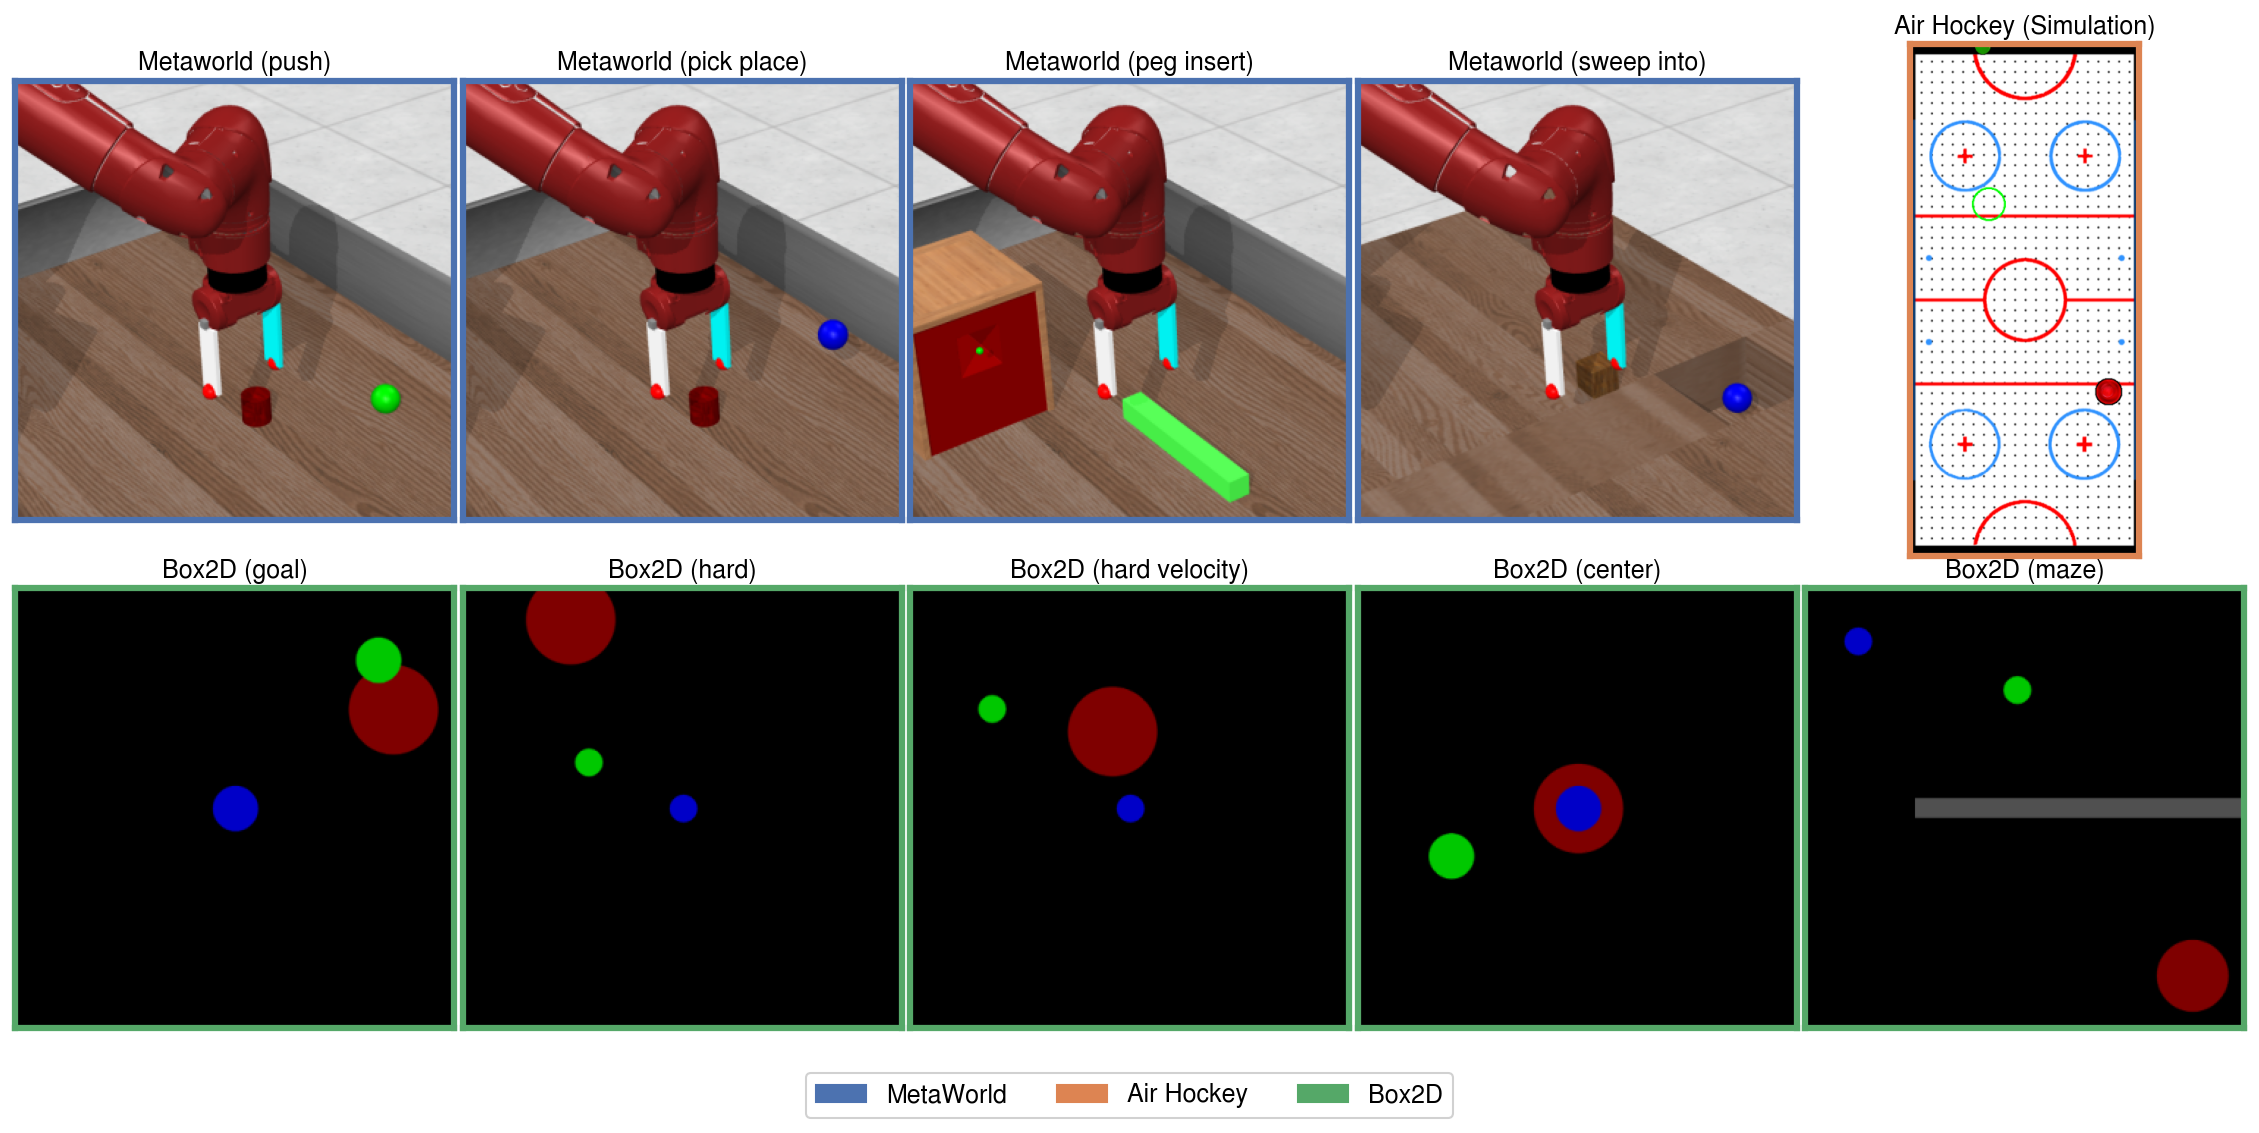
\includegraphics[width=\linewidth]{figure/task_set_figure.png}
        \caption{Task sets used in the simulation experiments.}
        \label{fig:task_set}
    \end{minipage}%
    \begin{minipage}[t]{0.25\textwidth}
        \centering
        \vspace{0pt}
        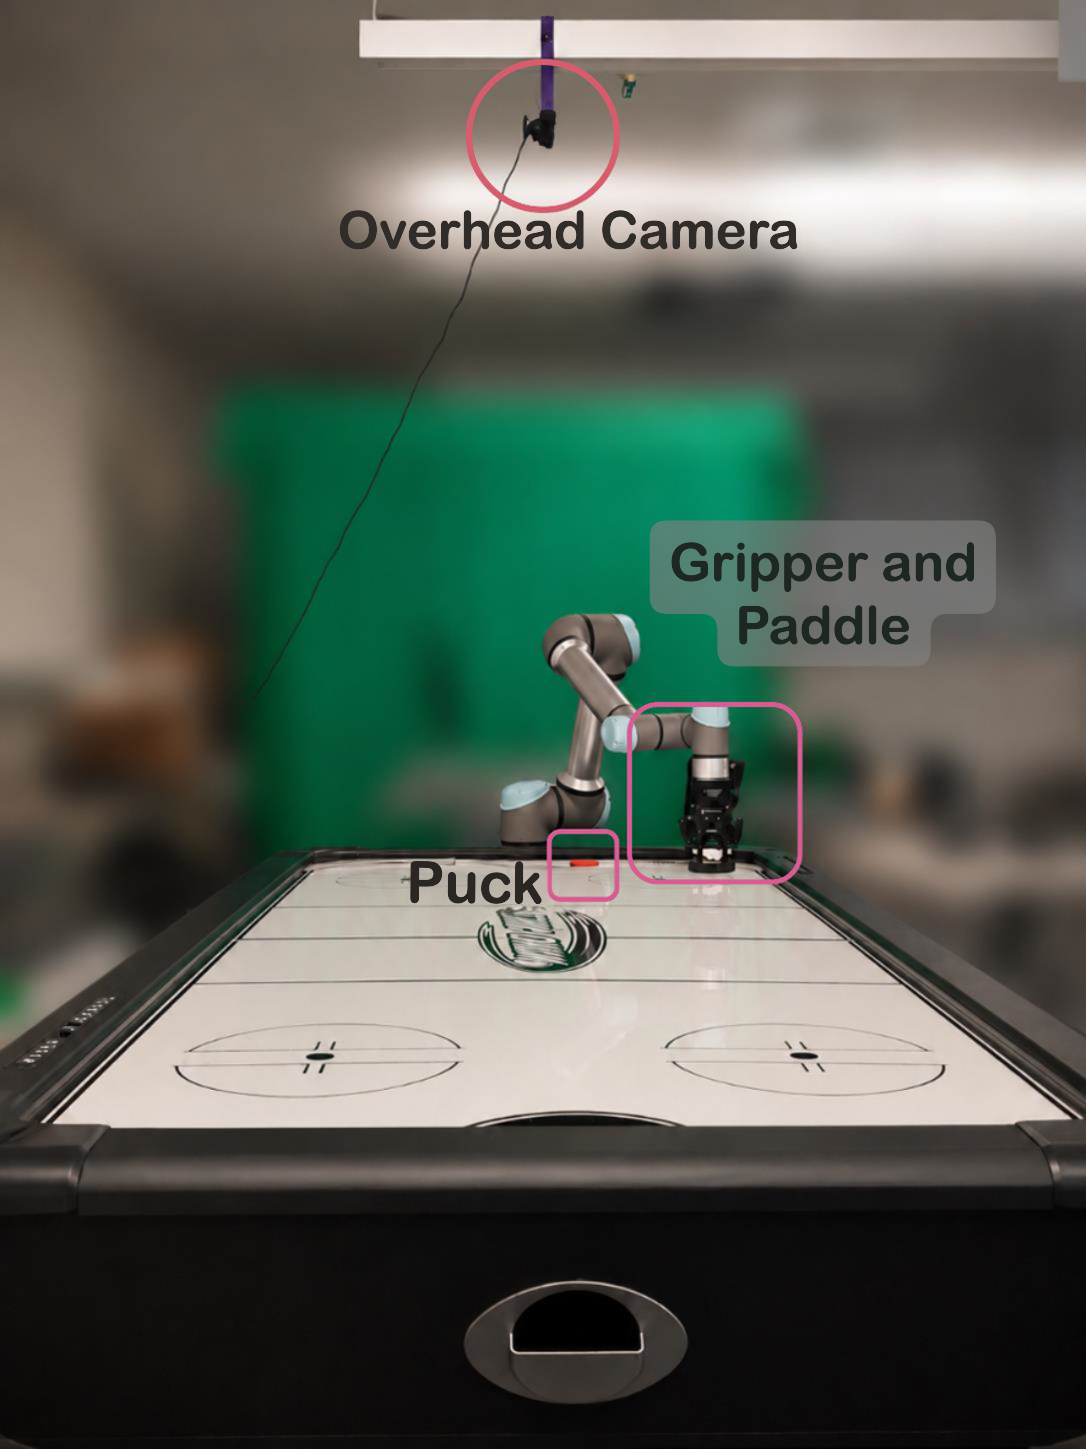
\includegraphics[width=\linewidth]{figure/air_hockey_setup.png}
        \caption{Real-world robotic air hockey testbed.}
        \label{fig:real_world_air_hockey_setup}
    \end{minipage}
    \vspace{-1em}
\end{figure}
All environments are wrapped as goal-conditioned vector environments.  Each
wrapper exposes a state vector $s_t$, achieved goal $g_t^{\mathrm{ach}}$,
desired goal $g_t^{\mathrm{des}}$, action $a_t$, and boolean success flag.  CRL
methods use future achieved goals for contrastive relabeling; sparse-reward
baselines use the same success flag as reward.  Episodes are automatically
reset in the vectorized training environment.

% \begin{table}[h]
% \centering
% \small
% \setlength{\tabcolsep}{5pt}
% \caption{Backend-level simulation settings.}
% \label{tab:appendix-backend-simulation}
% \begin{tabular}{p{0.24\linewidth}p{0.18\linewidth}p{0.22\linewidth}p{0.24\linewidth}}
% \toprule
% Backend & Train horizon & Termination on success & Vectorization \\
% \midrule
% Air Hockey & $300$ steps & yes & $256$ train envs \\
% Box2D & $400$ steps in paper launch & no & $256$ train envs \\
% MetaWorld & $150$ steps & yes & async, $256$ train envs \\
% \bottomrule
% \end{tabular}
% \end{table}

\subsection{Air Hockey}

The success radius from the goal state is $r_{\mathrm{goal}} = 0.06$. 
The paddle, puck, and goal are randomized at reset.  The wrapper terminates an
episode on success during training.  For the default physics tasks, episodes
also terminate if the puck hits the bottom or passes the paddle; out-of-bounds
termination is disabled.  For real-transfer, out-of-bounds termination is
enabled.

\begin{table}[h]
\centering
\small
\setlength{\tabcolsep}{5pt}
\caption{Default Air Hockey simulator parameters.}
\label{tab:appendix-air-hockey-default-physics}
\begin{tabular}{ll}
\toprule
Parameter & Value \\
\midrule
Simulator & Box2D Air Hockey simulator \\
Table length / width & $1.9304$ / $0.8636$ \\
Render size & $360$ \\
Paddle radius & $0.0508$ \\
Puck radius & $0.03175$ \\
Paddle density / damping & $2500$ / $3$ \\
Puck density / damping & $250$ / $0.5$ \\
Gravity & $-0.5$ \\
Force scaling & $1000$ \\
Max force timestep & $100$ \\
Wall bounce scale & $0.02$ \\
Blocks / obstacles / targets & $0/0/0$ \\
Paddles / pucks & $1/1$ \\
Randomized paddle spawn & true \\
Goal radius & $0.06$ \\
\bottomrule
\end{tabular}
\end{table}

\begin{table}[h]
\centering
\small
\setlength{\tabcolsep}{5pt}
\caption{Air Hockey real-transfer physics and corruption settings.}
\label{tab:appendix-air-hockey-real-transfer}
\begin{tabular}{ll}
\toprule
Parameter & Value \\
\midrule
Observation type & history \\
Domain randomization & enabled \\
Randomized variables & paddle density, puck damping, gravity \\
Paddle density range & $[2250,3750]$ \\
Puck damping range & $[0.1335,0.2225]$ \\
Gravity range & $[-0.826,-0.496]$ \\
SysID gravity & $-0.661$ \\
SysID puck damping & $0.178$ \\
Paddle damping & $17$ \\
Force scaling & $0.99$ \\
Max force timestep & $10000$ \\
Puck density & $3000$ \\
Paddle / puck radius & $0.0508$ / $0.03175$ \\
Paddle restitution & $1.0$ \\
Side / end wall restitution & $0.99$ / $0.7$ \\
PID control & enabled \\
PID gains & $k_p=9000$, $k_d=50$, $k_i=0$ \\
History length & $2$ \\
Puck observation noise & enabled, std. $0.01$ \\
Random occlusion & enabled, start rate $0.05$ per step \\
Occlusion length weights & $[75,39,18,9,4,2,1]$ \\
Observation delay & enabled, $0.025$s \\
Action delay & disabled \\
Near-paddle puck spawn probability & $0.15$ \\
Near-paddle spawn offset & $[0.025,0.05]$ m \\
Near-paddle spawn speed & $[0.0,0.2]$ m/s \\
Linear top spawn speed & $[0.0,0.5]$ m/s \\
\bottomrule
\end{tabular}
\end{table}

\subsection{Box2D}

% Box2D tasks are provided through the local \texttt{ac\_infer} checkout.  The
% paper launch uses fixed limits, reward aggregation \texttt{max}, and a horizon
% of $400$ steps for all Box2D paper-core tasks.  Success does not terminate the
% episode in the paper-core Box2D launch, which makes success-tick comparisons
% well-defined over the full horizon.

% The wrapped state is
% \[
%     s =
%     [x_c,y_c,\dot{x}_c,\dot{y}_c,\;
%       x_o,y_o,\dot{x}_o,\dot{y}_o],
% \]
% where $c$ is the controllable body and $o$ is the target/object body.  The
% achieved and desired goals are read from the underlying Box2D environment info
% dictionary.  For interaction-aware sampling, the source position is
% $(x_c,y_c)$ and the target position is $(x_o,y_o)$.

% \begin{table}[h]
% \centering
% \small
% \setlength{\tabcolsep}{5pt}
% \caption{Box2D paper-core tasks.}
% \label{tab:appendix-box2d-tasks}
% \begin{tabular}{p{0.15\linewidth}p{0.39\linewidth}p{0.34\linewidth}}
% \toprule
% Paper task name & Environment id & Variant \\
% \midrule
% Box2D center & \texttt{Box2dCenterCtrlTarget-v0} & \texttt{center-ctrl-target} \\
% Box2D goal & \texttt{Box2dGoalCtrlTarget-v0} & \texttt{goal-ctrl-target} \\
% Box2D hard & \texttt{Box2dGoalCtrlTargetHard-v0} & \texttt{goal-ctrl-target-hard} \\
% Box2D hard velocity & \texttt{Box2dGoalCtrlTargetHardVel-v0} & \texttt{goal-ctrl-target-hard-vel} \\
% Box2D maze & \texttt{Box2dMazeBallEasyNavigation-v0} & \texttt{maze-ball-easy-navigation} \\
% \bottomrule
% \end{tabular}
% \end{table}

The hard-velocity task is a local compatibility variant implemented in the
wrapper by taking \texttt{goal-ctrl-target-hard} and setting the target initial
velocity to $5.0$.

\subsection{MetaWorld}

MetaWorld tasks use compact point observations.  The state dimension is $7$:
\[
    s =
    [p_{\mathrm{hand}}\in\mathbb{R}^3,\;
      q_{\mathrm{gripper}}\in\mathbb{R},\;
      p_{\mathrm{object}}\in\mathbb{R}^3].
\]
Default goal gripper opening is $0.4$ and default hand offset is
$(0,0,0.03)$.  The default minimum distance
between the initial object and sampled goal is $0.15$.  Episodes terminate on
success during training.

\begin{table}[h]
\centering
\small
\setlength{\tabcolsep}{5pt}
\caption{MetaWorld paper-core tasks and success definitions.}
\label{tab:appendix-metaworld-tasks}
\begin{tabular}{p{0.23\linewidth}p{0.23\linewidth}p{0.22\linewidth}p{0.26\linewidth}}
\toprule
Paper task name & Env id & Achieved object & Success condition \\
\midrule
MetaWorld push & \texttt{push-v2} & object position & distance $<0.05$ \\
MetaWorld pick place & \texttt{pick-place-v2} & object position & distance $<0.07$ \\
MetaWorld peg insert & \texttt{peg-insert-side-v2} & peg head position & scaled distance $<0.07$ \\
MetaWorld sweep into & \texttt{sweep-into-v2} & object position & distance $<0.05$ and $z$ error $<0.02$ \\
\bottomrule
\end{tabular}
\end{table}

The \texttt{peg-insert-side-v2} wrapper maps to the canonical
\texttt{peg-insert-side-v3} task, uses success scale $(1,2,2)$, and uses a
goal hand offset $(0.13,0,0.03)$.  The \texttt{sweep-into-v2} success
calculation ignores the target $z$ axis for the main distance while enforcing a
separate $z$-axis threshold of $0.02$.

\subsection{Post-Hoc Air Hockey Consecutive Evaluation}

For the one-minute Air Hockey challenge, evaluation is separate from training.
The evaluator disables terminate-on-success so the puck can be re-armed to a
new goal after each success.  The standard setting is
\[
    \text{horizon}=1200\text{ steps},\qquad
    \text{seeds}=1,\ldots,16.
\]
The recorded metrics are complete rate, mean number of consecutive goals, and
maximum number of consecutive goals.  Rendering is disabled by default for
batch evaluation, but the same evaluator can render rollout videos for selected
checkpoints.


